%State Chart Syntax
\section{Syntax of \plcchart}
\label{sec:statechartsyn}

Abstract syntax of \plcchart language:
\begin{definition}
\plcchart

\begin{itemize}
	\item Eq := $\;$ \boldmath$=$\unboldmath $\; \mid \;$ \boldmath$\neq$\unboldmath $\; \mid \;$ \boldmath$<$\unboldmath $\; \mid \;$ \boldmath$\leq$\unboldmath $\; \mid \;$ \boldmath$>$\unboldmath $\; \mid \;$ \boldmath$\geq$\unboldmath	
	\item Op := $\;$ \boldmath$+$\unboldmath $\; \mid \;$ \boldmath$-$\unboldmath $\; \mid \;$ \boldmath$*$\unboldmath $\; \mid \;$ \boldmath$/$\unboldmath $\; \mid \;$ \boldmath$\%$\unboldmath $\; \mid \;$ \boldmath$\&\&$\unboldmath $\; \mid \;$ \textbf{\texttt{||}} $\; \mid \;$ \boldmath$\mathbin{\char`\^}$\unboldmath

	\item Expression := Expression Op Expression $\mid$ Op Expression $\mid$ Var $\mid$ \textbf{Constant}
	
	\item Type := \textbf{Char} $\mid$ \textbf{Int} $\mid$ \textbf{Long} $\mid$ \textbf{Bool} $\mid$ \textbf{Float}
	\item Var := $\mathbf{v_0 \mid v_1 \mid v_2 \mid ... \mid v_n}$

	\item Condition := Expression Eq Expression $\mid$ Var

		
	\item StoreBlock := Type \textbf{Identifier} = Expression $\mid$ Type \textbf{Identifier} = Expresion; StoreBlock
	\item DelayBlock := Expression
	\item OutputBlock := \textbf{Identifier}
	\item InputBlock := Type \textbf{Identifier}
	\item Block := StoreBlock $\mid$ OutputBlock $\mid$ DelayBlock $\mid$ InputBlock

	
	\item Transition := Block Condition Block
	
	\item Program := StartBlock Condition Block $\mid$ Transition
\end{itemize}
\end{definition}

\begin{figure}[htp]
    \centering
    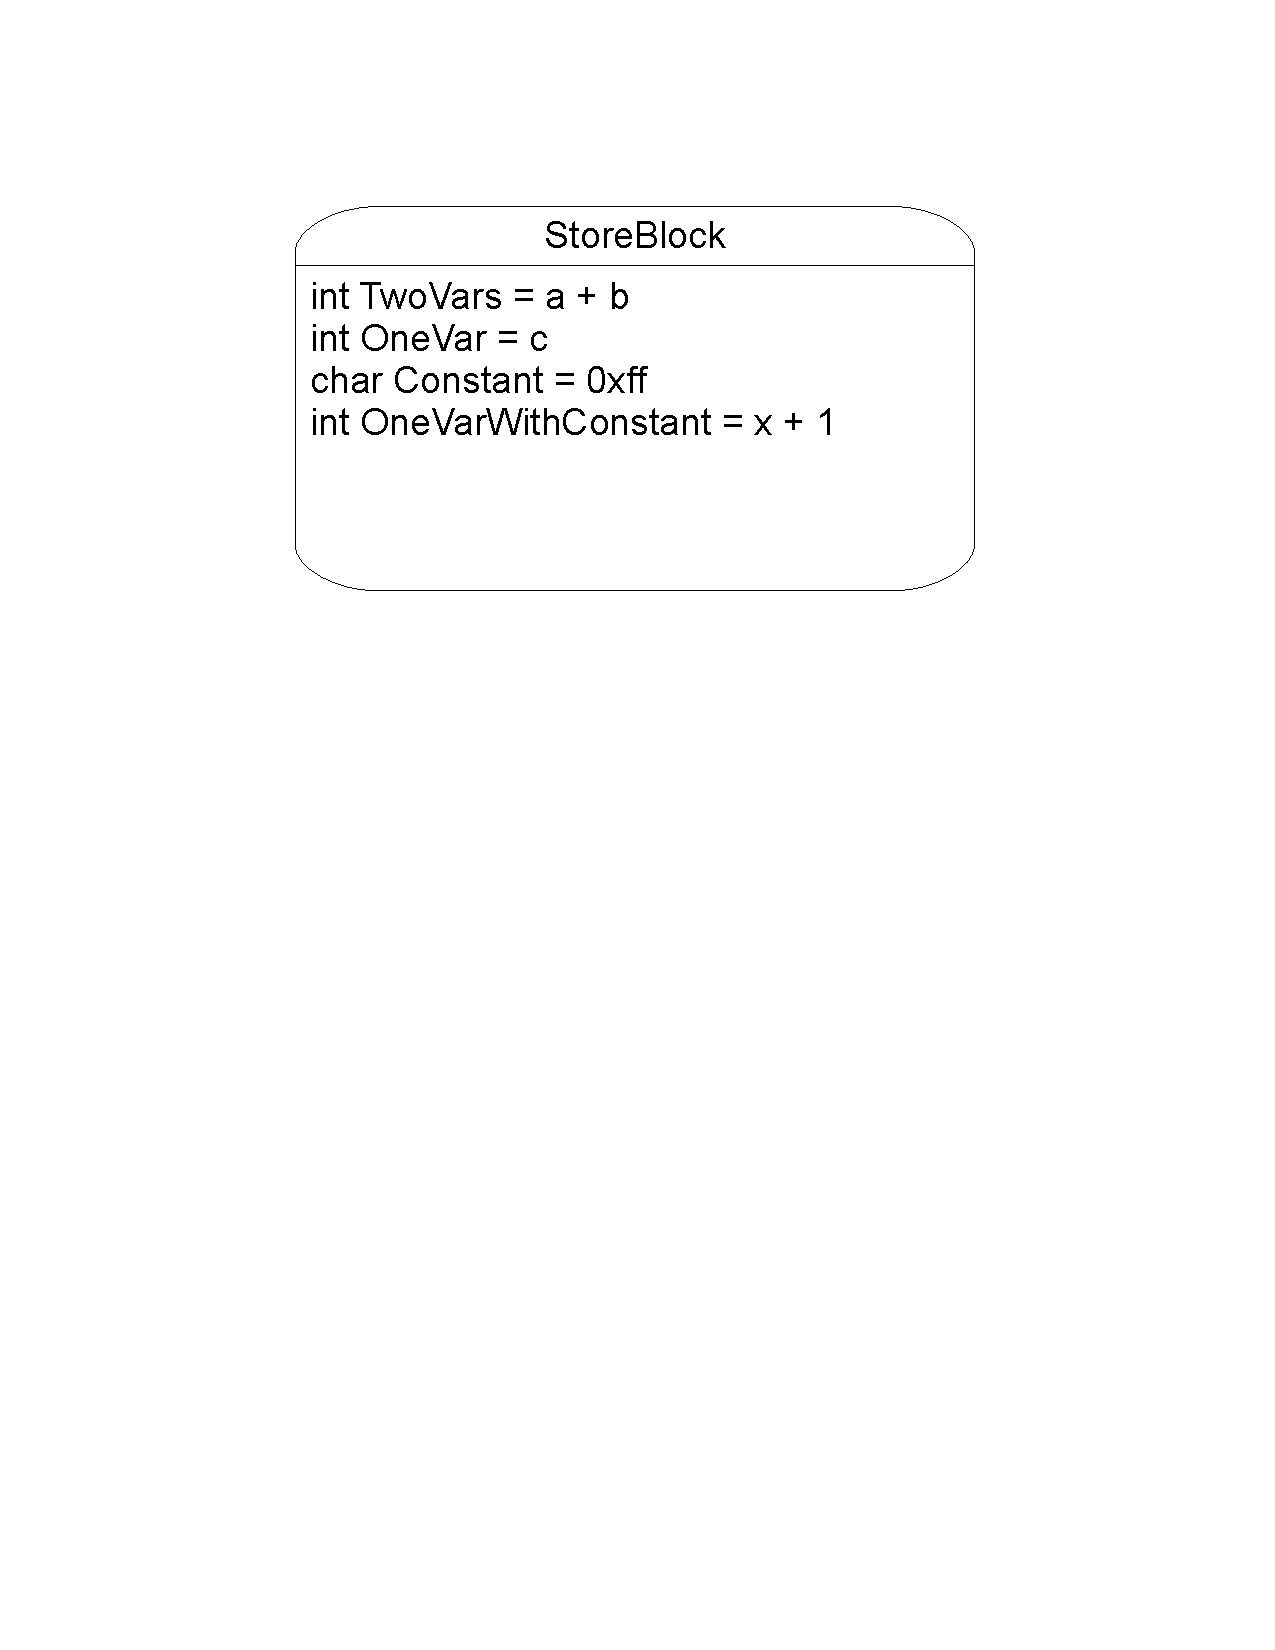
\includegraphics[trim= 20mm 175mm 20mm 10mm, clip, width=\imgmedium]{./images/state_storeblock.pdf}
    \caption{Example Of A Store Block As Implemented In PLCEdit}
    \label{fig:state_storeblock}
\end{figure}

In figure \ref{fig:state_storeblock} we see a store block represented as it would be drawn in the tool. Each line of a store block has the format shown in our abstract syntax. A line consists of a type (which in figure \ref{fig:state_storeblock} we have int, and char) an identifier, the equals symbol, and a value. A value can take the form of several expressions as show in figure \ref{fig:state_storeblock}. Our abstract syntax also allows for many lines to occur in each StoreBlock. This basic design choice allows formulae to be computed much easier in sequence rather than have several blocks to perform one set of operations.

Transitions in our system must start from an initial block object and must terminate at another block. Transitions must be mutually exclusive to be valid that is for all edges leaving the block conditions formed by expressions $E_1, E_2, E_3...E_n$: $\forall(i \neq j \rightarrow E_i \cap E_j = \emptyset)$. In addition given a set of conditions $E_1 \cup E_2 \cup E_3 \cup ... \cup E_n = \mathbb{U}$. In simpler terms all transition conditions must be mutually exclusive and must cover the entire space. It is an error in our language if you have a condition that can occur that is not explicitly described. It is valid to have a transition begin and terminate from the same block. 

\begin{figure}[htp]
    \centering
    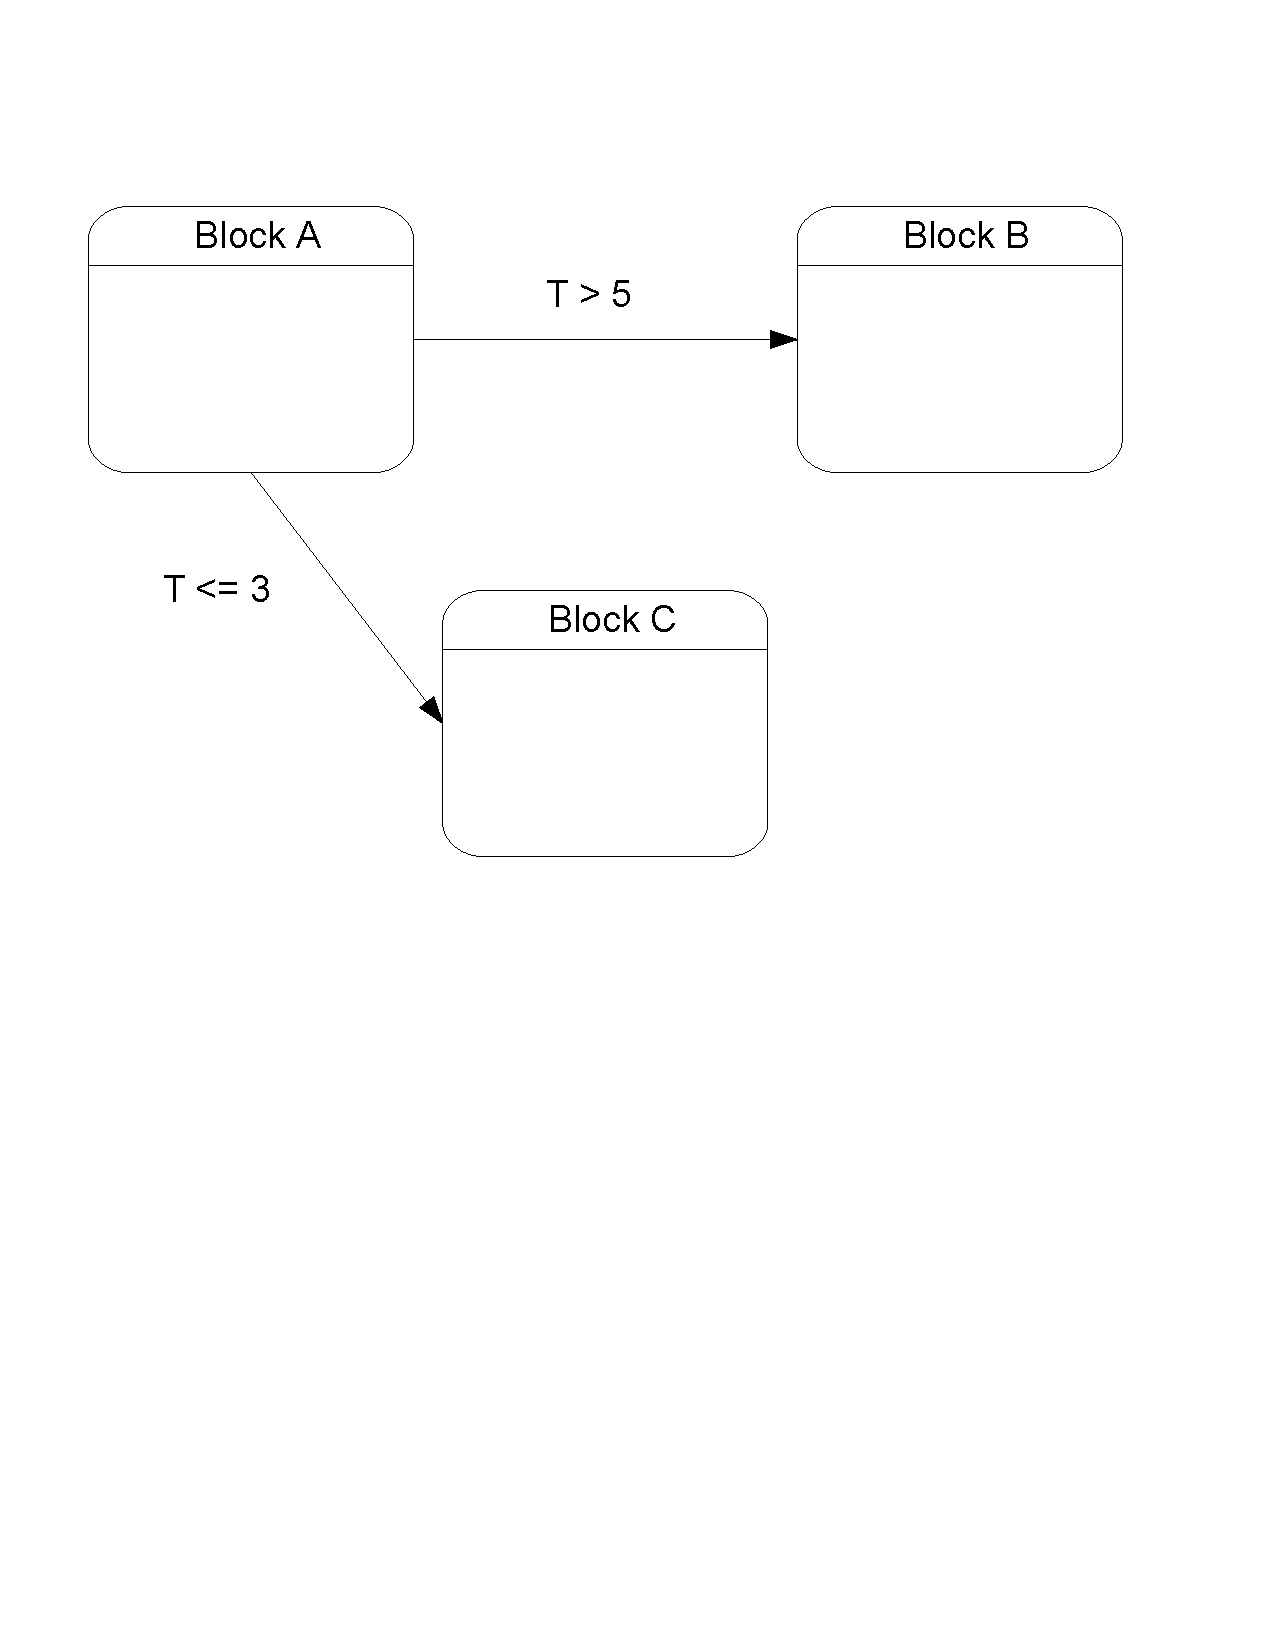
\includegraphics[trim= 10mm 130mm 20mm 10mm, clip, width=\imgmedium]{./images/state_transition.pdf}
    \caption{Example of Basic Transitions}
    \label{fig:state_transition}
\end{figure}




